\documentclass{ctexart}
    \usepackage{mathrsfs}
    \usepackage{multirow}
    \usepackage{graphicx}
    \usepackage{array}
    \usepackage{makecell}
    \usepackage{amsmath}
    \usepackage{booktabs}
    \usepackage{float}
    \newcommand\mgape[1]{\gape{$\vcenter{\hbox{#1}}$}}

    \author{钱思天\ 1600011388 No.8}
    \title{实验八:测量金属的杨氏模量\ 实验报告}
    \begin{document}
      \maketitle
      \section{实验数据与处理}
      \subsection{多次测量物理量数据处理}
      \subsubsection{利用CCD测量金属的杨氏模量}
      % Table generated by Excel2LaTeX from sheet 'Sheet1'
\begin{table}[H]
    \centering
    \caption{所用砝码组质量}
    \resizebox{\textwidth}{!}
    {
      \begin{tabular}{lcccccccccc}
      砝码编号 $i$ & 0     & 1     & 2     & 3     & 4     & 5     & 6     & 7     & 8     & 9 \\
      砝码质量 $m_i /g$ & 99.97 & 199.94 & 200.00 & 199.98 & 199.98 & 199.91 & 199.92 & 200.05 & 199.50 & 200.07 \\
      \end{tabular}%
    }
    \label{tab:addlabel}%
  \end{table}%
  % Table generated by Excel2LaTeX from sheet 'Sheet1'
\begin{table}[H]
    \centering
    \caption{所测金属丝直径}
    \resizebox{\textwidth}{!}
    {
      \begin{tabular}{lrrrrrrrrrr}
      所测直径 & \multicolumn{1}{l}{$d_1$} & \multicolumn{1}{l}{$d_2$} & \multicolumn{1}{l}{$d_3$} & \multicolumn{1}{l}{$d_4$} & \multicolumn{1}{l}{$d_5$} & \multicolumn{1}{l}{$d_6$} & \multicolumn{1}{l}{$d_7$} & \multicolumn{1}{l}{$d_8$} & \multicolumn{1}{l}{$d_9$} & \multicolumn{1}{l}{$d_{10}$} \\
      读数$d_i/mm$    & 0.315 & 0.316 & 0.312 & 0.316 & 0.312 & 0.315 & 0.316 & 0.315 & 0.316 & 0.317 \\
      \end{tabular}%
    }
    \label{tab:addlabel}%
  \end{table}%
% Table generated by Excel2LaTeX from sheet 'Sheet1'
\begin{table}[H]
    \centering
    \caption{逐个依次添加砝码所得横线位置}
    \resizebox{\textwidth}{!}
    {
      \begin{tabular}{ccccccc}
      \multicolumn{1}{l}{次数 $i$} & \multicolumn{1}{l}{增加砝码质量 $\Delta m_i /g$} & \multicolumn{1}{l}{砝码总质量 $m_i /g$} & \multicolumn{1}{l}{增添位置 $r/mm$} & \multicolumn{1}{l}{减少位置 $r'/mm$} & \multicolumn{1}{l}{平均位置 $\bar{r}/mm$} & \multicolumn{1}{l}{逐差长度 $\delta L/mm$} \\
      0     & 99.97 & 99.97 & 2.86  & 2.87  & 2.87  & 0.60  \\
      1     & 199.94 & 299.91  & 2.97  & 2.98  & 2.98  & 0.60  \\
      2     & 200.00 & 499.91  & 3.09  & 3.1   & 3.10  & 0.59  \\
      3     & 199.98 & 699.89  & 3.23  & 3.23  & 3.23  & 0.58  \\
      4     & 199.98 & 899.87  & 3.36  & 3.35  & 3.36  & 0.57  \\
      5     & 199.91 & 1099.78  & 3.47  & 3.46  & 3.47  & -- \\
      6     & 199.92 & 1299.70  & 3.57  & 3.58  & 3.58  & -- \\
      7     & 200.05 & 1499.75  & 3.68  & 3.69  & 3.69  & -- \\
      8     & 199.50 & 1699.25  & 3.80  & 3.81  & 3.81  & -- \\
      9     & 200.07 & 1899.32  & 3.92  & 3.92  & 3.92  & -- \\
      \end{tabular}%
    }
    \label{tab:addlabel}%
  \end{table}%
  \subsubsection{利用光杠杆法测量杨氏模量}
  % Table generated by Excel2LaTeX from sheet 'Sheet2'
\begin{table}[H]
  \centering
  \caption{所用砝码组质量}
  \resizebox{\textwidth}{!}
  {
    \begin{tabular}{lcccccccccc}
    砝码编号 $i$& 1     & 2     & 3     & 4     & 5     & 6     & 7     & 8     & 9&10 \\
    砝码质量 $\Delta m_i /g$ & 195.46 & 200.26 & 199.72 & 199.65 & 199.71 & 199.83 & 199.88 & 199.80 & 199.86 & 200.03 \\
    \end{tabular}%
  }
  \label{tab:addlabel}%
\end{table}%
% Table generated by Excel2LaTeX from sheet 'Sheet2'
\begin{table}[H]
  \centering
  \caption{所测金属丝直径}
   
      \resizebox{\textwidth}{!}
      {
        \begin{tabular}{lrrrrrrrrrr}
    所测直径 & \multicolumn{1}{l}{$d_1$} & \multicolumn{1}{l}{$d_2$} & \multicolumn{1}{l}{$d_3$} & \multicolumn{1}{l}{$d_4$} & \multicolumn{1}{l}{$d_5$} & \multicolumn{1}{l}{$d_6$} & \multicolumn{1}{l}{$d_7$} & \multicolumn{1}{l}{$d_8$} & \multicolumn{1}{l}{$d_9$} & \multicolumn{1}{l}{$d_{10}$} \\
    读数  $d_i/mm$  & 0.325 & 0.320  & 0.321 & 0.320  & 0.318 & 0.317 & 0.319 & 0.317 & 0.316 & 0.314 \\
    \end{tabular}%
      }
  \label{tab:addlabel}%
\end{table}%
% Table generated by Excel2LaTeX from sheet 'Sheet1'
\begin{table}[H]
  \centering
  \caption{逐个依次添加砝码所得卡丝位置}
  \resizebox{\textwidth}{!}
  {
    \begin{tabular}{ccrcccc}
    \multicolumn{1}{l}{次数 $i$} & \multicolumn{1}{l}{本次添加砝码质量 $\Delta m_i /g$} & \multicolumn{1}{l}{砝码总重量 $m_i /g$} & \multicolumn{1}{l}{正向位置 $r/cm$} & \multicolumn{1}{l}{反向位置 $r'/cm$} & \multicolumn{1}{l}{平均位置 $\bar{r}/cm$} & \multicolumn{1}{l}{逐差长度 $\delta L/cm$} \\
    0     & 99.97 & 99.97 & 2.86  & 2.87  & 2.87  & 0.60  \\
    1     & 199.94 & 299.91  & 2.97  & 2.98  & 2.98  & 0.60  \\
    2     & 200.00 & 499.91  & 3.09  & 3.1   & 3.10  & 0.59  \\
    3     & 199.98 & 699.89  & 3.23  & 3.23  & 3.23  & 0.58  \\
    4     & 199.98 & 899.87  & 3.36  & 3.35  & 3.36  & 0.57  \\
    5     & 199.91 & 1099.78  & 3.47  & 3.46  & 3.47  & -- \\
    6     & 199.92 & 1299.70  & 3.57  & 3.58  & 3.58  & -- \\
    7     & 200.05 & 1499.75  & 3.68  & 3.69  & 3.69  & -- \\
    8     & 199.50 & 1699.25  & 3.80  & 3.81  & 3.81  & -- \\
    9     & 200.07 & 1899.32  & 3.92  & 3.92  & 3.92  & -- \\
    \end{tabular}%
  }
  \label{tab:addlabel}%
\end{table}%
\subsubsection{梁的弯曲测量杨氏模量}
% Table generated by Excel2LaTeX from sheet 'Sheet3'
\begin{table}[H]
  \centering
  \caption{实验所用砝码组}
    \begin{tabular}{lcccccc}
    砝码编号 $i$ & 1     & 2     & 3     & 4     & 5     & 6 \\
    砝码质量 $\Delta m_i /g$ & 200.11 & 200.81 & 200.03 & 200.11 & 200.57 & 200.14 \\
    \end{tabular}%
  \label{tab:addlabel}%
\end{table}%
% Table generated by Excel2LaTeX from sheet 'Sheet3'
\begin{table}[H]
  \centering
  \caption{梁的宽度}
    \begin{tabular}{lcccccc}
    宽度$a_i/mm$ & \multicolumn{1}{l}{$a_1$} & \multicolumn{1}{l}{$a_2$} & \multicolumn{1}{l}{$a_3$} & \multicolumn{1}{l}{$a_4$} & \multicolumn{1}{l}{$a_5$} & \multicolumn{1}{l}{$a_6$} \\
    读数    & 9.94  & 9.92  & 9.90  & 9.84  & 9.86  & 9.84  \\
    \end{tabular}%
  \label{tab:addlabel}%
\end{table}%
% Table generated by Excel2LaTeX from sheet 'Sheet3'
\begin{table}[H]
  \centering
  \caption{梁的厚度}
    \begin{tabular}{lrrrrrr}
    厚度$h_i/mm$ & \multicolumn{1}{l}{$h_1$} & \multicolumn{1}{l}{$h_2$} & \multicolumn{1}{l}{$h_3$} & \multicolumn{1}{l}{$h_4$} & \multicolumn{1}{l}{$h_5$} & \multicolumn{1}{l}{$h_6$} \\
    读数    & 1.499 & 1.521 & 1.532 & 1.519 & 1.541 & 1.539 \\
    \end{tabular}%
  \label{tab:addlabel}%
\end{table}%
% Table generated by Excel2LaTeX from sheet 'Sheet3'
\begin{table}[H]
  \centering
  \caption{逐个依次添加砝码所得梁最低点位置}
  \resizebox{\textwidth}{!}
  {
    \begin{tabular}{ccccccc}
    \multicolumn{1}{l}{次数 $i$} & \multicolumn{1}{l}{本次添加砝码质量 $\Delta m_i /g$} & \multicolumn{1}{l}{砝码总重量 $m_i /g$} & \multicolumn{1}{l}{正向位置 $\lambda /mm$} & \multicolumn{1}{l}{反向位置$\lambda '/mm$} & \multicolumn{1}{l}{平均位置 $\bar{\lambda}/mm$} & \multicolumn{1}{l}{逐差长度 $\delta \Lambda/mm$} \\
    1     & 200.11 & 200.11 & 37.585 & 37.460 & 37.523 & -2.458  \\
    2     & 200.81 & 400.92  & 36.770 & 36.692 & 36.731 & -2.503  \\
    3     & 200.03 & 600.95  & 35.932 & 35.827 & 35.880 & -2.503  \\
    4     & 200.11 & 801.06  & 35.111 & 35.018 & 35.065 & -- \\
    5     & 200.57 & 1001.63  & 34.271 & 34.185 & 34.228 & -- \\
    6     & 200.14 & 1201.77  & 33.422 & 33.332 & 33.377 & -- \\
    \end{tabular}%
  }
  \label{tab:addlabel}%
\end{table}%
\subsection{一次测量物理量测量数值及其不确定度}
\subsubsection{利用CCD测量金属的杨氏模量}
在本实验中,一次测量物理量分别是铁丝的长度,以及螺旋测微计的零点位置。利用公式:
$$\sigma=\frac{e}{\sqrt{3}}$$
及实际测量数据可得下表:
% Table generated by Excel2LaTeX from sheet 'Sheet1'
\begin{table}[H]
  \centering
  \caption{本实验中一次测量物理量及其不确定度}
  
    \begin{tabular}{lllr}
    物理量   & 铁丝长度$L \pm \sigma_L /cm$ & 螺旋测微计零点读数$d_0 \pm \sigma_d /mm$ &  \\
    值     & 80.41 $\pm$ 0.06 & $-$0.003$\pm$0.002 &  \\
    \end{tabular}%
  \label{tab:addlabel}%
\end{table}%
\subsubsection{利用光杠杆测量金属的杨氏模量}
在本实验中,一次测量物理量分别是铁丝的长度,螺旋测微计的零点位置,光杠杆臂长以及望远镜的工作距离。利用公式:
$$\sigma=\frac{e}{\sqrt{3}}$$
及实际测量数据可得下表:
% Table generated by Excel2LaTeX from sheet 'Sheet2'
\begin{table}[H]
  \centering
  \caption{本实验中一次测量物理量及其不确定度}
  \resizebox{\textwidth}{!}
  {
    \begin{tabular}{lllll}
    物理量   & 铁丝长度$L \pm \sigma_L /cm$ & 螺旋测微计零点读数$d_0 \pm \sigma_d /mm$ & 工作距离$R \pm \sigma_R /cm $ & 光杠杆臂长$D \pm \sigma_D /cm$ \\
    数值    & 77.60$\pm$0.06 & $-$0.003$\pm$0.002 & 136.49 $\pm$ 0.06 & 9.20$\pm$0.01 \\
    \end{tabular}%
  }
  \label{tab:addlabel}%
\end{table}%
\subsubsection{梁的弯曲测量杨氏模量}
在本实验中,一次测量物理量分别是金属梁的有效长度及螺旋测微计的零点位置。利用公式:
$$\sigma=\frac{e}{\sqrt{3}}$$
及实际测量数据可得下表:
% Table generated by Excel2LaTeX from sheet 'Sheet3'
\begin{table}[htbp]
  \centering
  \caption{本实验中一次测量物理量及其不确定度}
    \begin{tabular}{lll}
    物理量   & 金属梁有效长度$L\pm \sigma_L/cm$ & 螺旋测微计零点读数$h_0 \pm \sigma_h /mm$ \\
    数值    & 23.32$\pm$0.01 & $-$0.021$\pm$0.02 \\
    \end{tabular}%
  \label{tab:addlabel}%
\end{table}%
\subsection{用逐差法和最小二乘法处理数据}
\subsubsection{利用CCD测量金属的杨氏模量}
根据前文所展示的实验数据,可作$\bar{r}$与$m$关系图如下:
\begin{figure}[H]
  \centering
  \caption{本实验中$\bar{r}$与$m$数据图}
  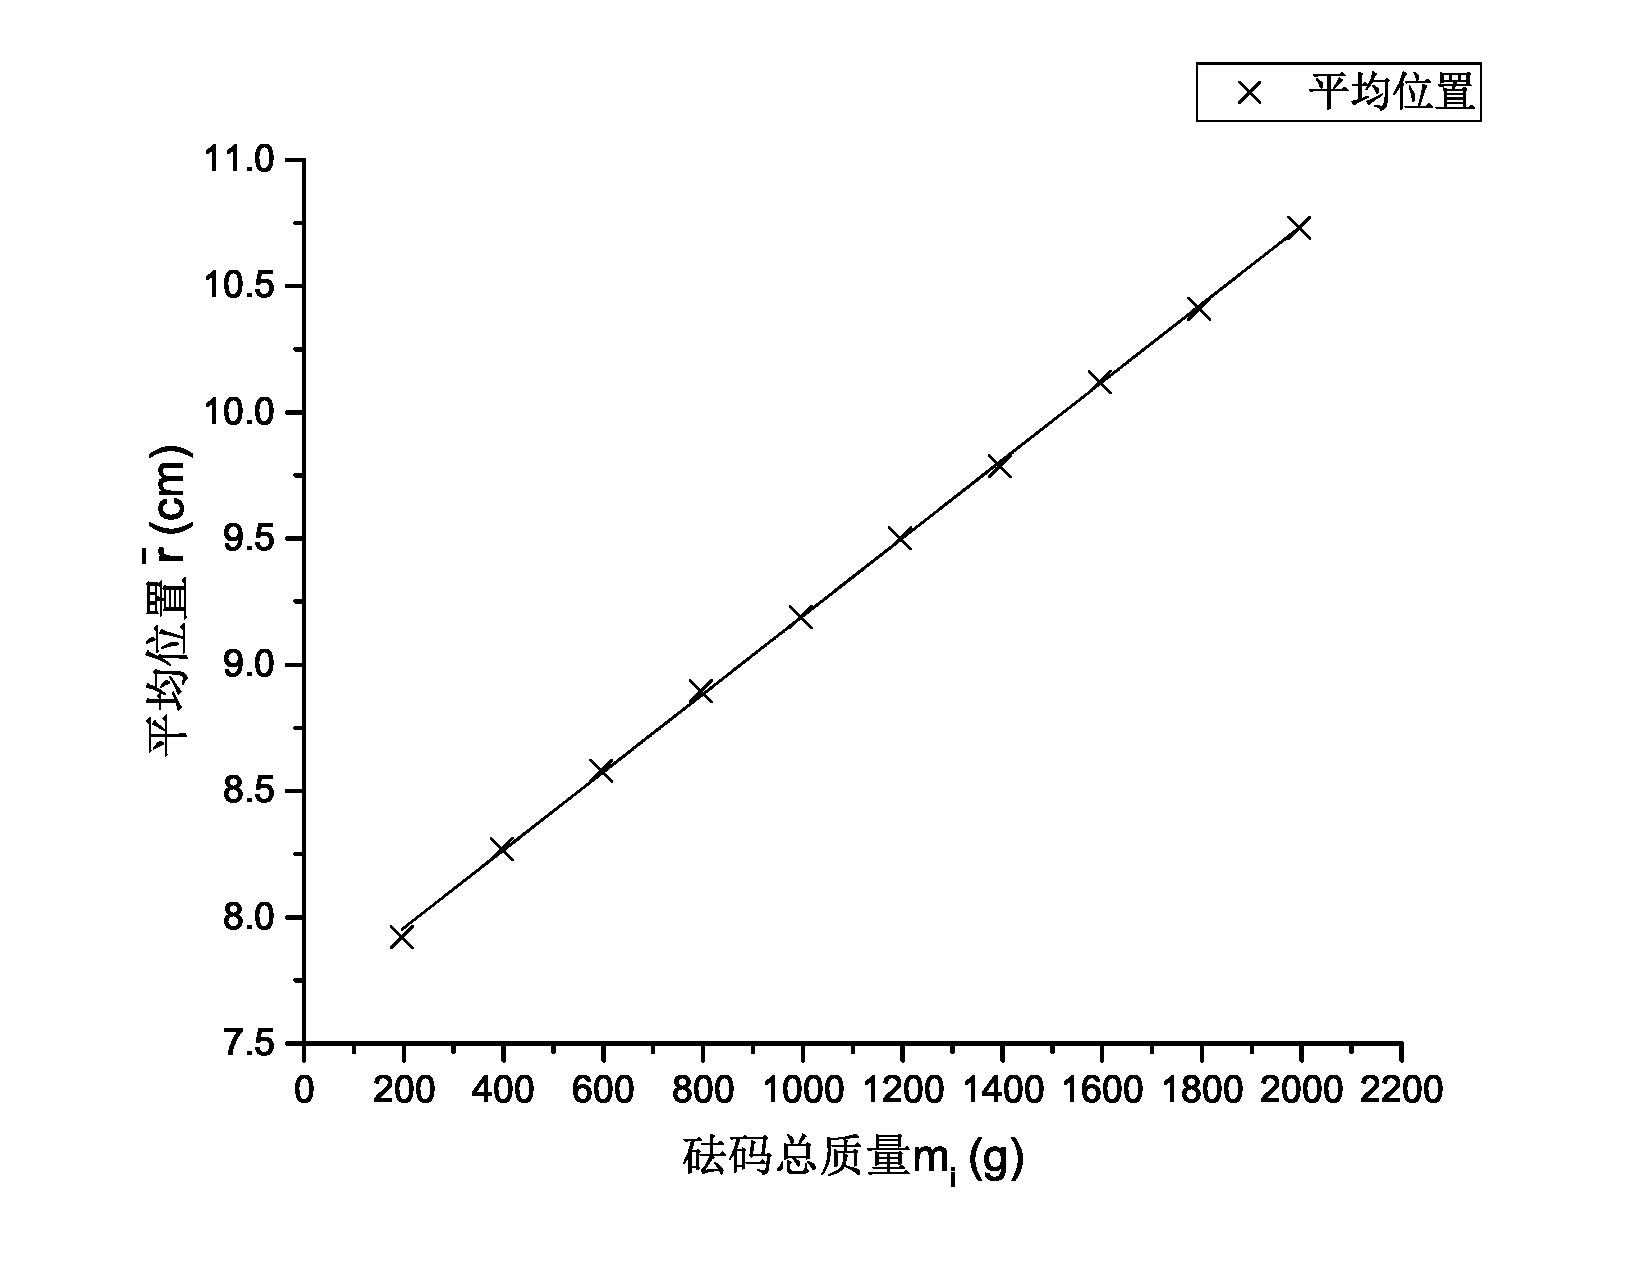
\includegraphics[width=\textwidth]{2}
  \label{fig:digit}
\end{figure}
从图中可以看出,$\bar{r}$与$m$成基本呈线性关系,计算得$r\approx 0.999$,故确实存在线性关系,下面分别用逐差法和最小二乘法进行数据处理。
\paragraph{逐差法}之前的数据处理中已经计算了各次逐差的值,列表如下:
% Table generated by Excel2LaTeX from sheet 'Sheet1'
\begin{table}[H]
  \centering
  \caption{逐差结果数据表}
    \begin{tabular}{lccccc}
    逐差次数  & \multicolumn{1}{l}{$\bar{r}_5-\bar{r}_0$} & \multicolumn{1}{l}{$\bar{r}_6-\bar{r}_1$} & \multicolumn{1}{l}{$\bar{r}_7-\bar{r}_2$} & \multicolumn{1}{l}{$\bar{r}_8-\bar{r}_3$} & \multicolumn{1}{l}{$\bar{r}_9-\bar{r}_4$} \\
    逐差长度 $\delta L_i/mm$ & 0.60  & 0.60  & 0.59  & 0.58  & 0.57  \\
    \end{tabular}%
  \label{tab:addlabel}%
\end{table}%
利用公式,有:
$$\delta L=\frac{1}5 \sum_{i=1}^5{\delta L_i}=0.588(mm)$$
下计算不确定度:
A类:$$\sigma_{\bar{L}}=\sqrt{\frac{\sum\limits_{i=1}^5{(\delta L_i-\overline{\delta L})^2}}{5\times4}}=0.006(mm)$$
B类:$$e_L=\sum\limits_{i=1}^5{\frac{e+e}5}=0.02(mm)\Rightarrow \sigma=\frac{e}{\sqrt{3}}=0.012(mm)$$
总不确定度:$$\sigma_L=\sqrt{\sigma^2+\sigma_{\bar{L}}^2}=0.013(mm)$$
综上,得;$$\delta L\pm \sigma_L=0.588\pm 0.013(mm)$$
\paragraph{最小二乘法}
设$$\bar{r}=k\times m+b$$
考虑到需要计算的物理量,我们对截距进行分析:
$$k=\frac{\sum\limits_{i=0}^9{(\bar{r}_i-\bar{r})(m_i-\bar{m})}}{\sum\limits_{i=0}^9{(m_i-\bar{m})^2}}=5.88\times 10^{-4}(mm/g)$$
下计算不确定度:
首先计算$\bar{r}$的不确定度:
A类:$$\sigma_r =\sqrt{\frac{1-r^2}{10-2}\sum\limits_{i=0}^9{(\bar{r}_i-\bar{r})^2}}=0.009(mm)$$
B类:$$\sigma=\frac{e+e}{\sqrt{3}}=0.012(mm)$$
总不确定度:$$\sigma_{\bar{r}}=\sqrt{\sigma^2+\sigma_r^2}=0.015(mm)$$
得$k$的不确定度:
$$\sigma_k=\frac{\sigma}{\sqrt{\sum\limits_{i=0}^9{(m_i-\bar{m})^2}}}=6\times10^{-6}(mm/g)$$
故:
$$k\pm \sigma_k=(5.88\pm 0.06  )\times 10^{-4}(mm/g)$$
\subsubsection{利用光杠杆测量金属的杨氏模量}
根据前文所展示的实验数据,可作$\bar{r}$与$m$关系图如下:
\begin{figure}[H]
  \centering
  \caption{本实验中$\bar{r}$与$m$数据图}
  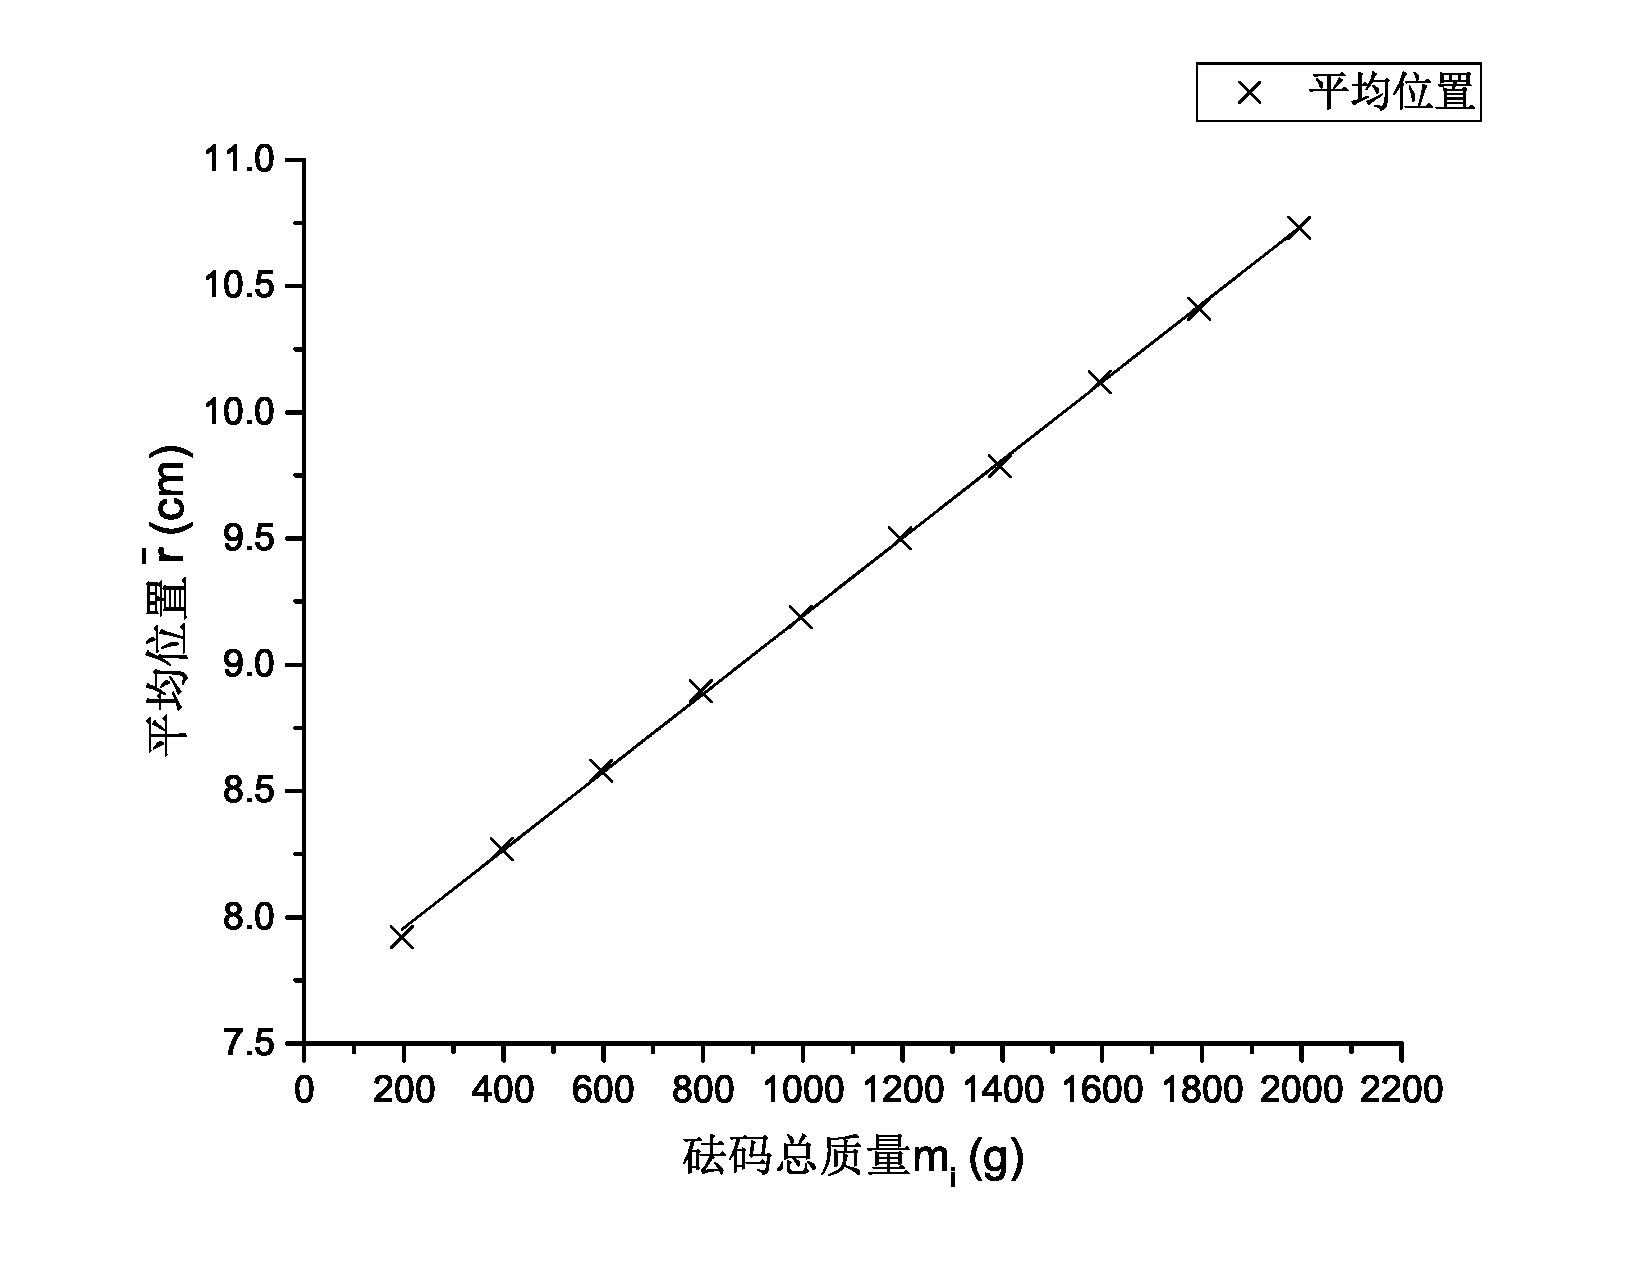
\includegraphics[width=\textwidth]{2}
  \label{fig:digit}
\end{figure}
从图中可以看出,$\bar{r}$与$m$成基本呈线性关系,计算得$r\approx 0.999$,故确实存在线性关系,下面分别用逐差法和最小二乘法进行数据处理。
\paragraph{逐差法}之前的数据处理中已经计算了各次逐差的值,列表如下:
% Table generated by Excel2LaTeX from sheet 'Sheet2'
\begin{table}[htbp]
  \centering
  \caption{逐差结果数据表}
    \begin{tabular}{lccccc}
    逐差次数  & \multicolumn{1}{l}{$\bar{r}_5-\bar{r}_0$} & \multicolumn{1}{l}{$\bar{r}_6-\bar{r}_1$} & \multicolumn{1}{l}{$\bar{r}_7-\bar{r}_2$} & \multicolumn{1}{l}{$\bar{r}_8-\bar{r}_3$} & \multicolumn{1}{l}{$\bar{r}_9-\bar{r}_4$} \\
    逐差长度 $\delta L/cm$ & 1.58  & 1.52  & 1.54  & 1.52  & 1.54  \\
    \end{tabular}%
  \label{tab:addlabel}%
\end{table}%

利用公式,有:
$$\delta L=\sum_{i=1}^5{\delta L_i}=1.540(cm)$$
下计算不确定度:
A类:$$\sigma_{\bar{L}}=\sqrt{\frac{\sum\limits_{i=1}^5{(\delta L_i-\overline{\delta L})^2}}{5\times4}}=0.011(cm)$$
B类:$$e_L=\sum\limits_{i=1}^5{\frac{e+e}5}=0.02(cm)\Rightarrow \sigma=\frac{e}{\sqrt{3}}=0.012(cm)$$
总不确定度:$$\sigma_L=\sqrt{\sigma^2+\sigma_{\bar{L}}^2}=0.016(cm)$$
综上,得;$$\delta L\pm \sigma_L=1.540\pm 0.016(cm)$$
\paragraph{最小二乘法}
设$$\bar{r}=k\times m+b$$
考虑到需要计算的物理量,我们对截距进行分析:
$$k=\frac{\sum\limits_{i=0}^9{(\bar{r}_i-\bar{r})(m_i-\bar{m})}}{\sum\limits_{i=0}^9{(m_i-\bar{m})^2}}=1.545\times 10^{-3}(cm/g)$$
下计算不确定度:
首先计算$\bar{r}$的不确定度:
A类:$$\sigma_r =\sqrt{\frac{1-r^2}{10-2}\sum\limits_{i=0}^9{(\bar{r}_i-\bar{r})^2}}=0.016(cm)$$
B类:$$\sigma=\frac{e+e}{\sqrt{3}}=0.012(cm)$$
总不确定度:$$\sigma_{\bar{r}}=\sqrt{\sigma^2+\sigma_r^2}=0.020(cm)$$
得$k$的不确定度:
$$\sigma_k=\frac{\sigma}{\sqrt{\sum\limits_{i=0}^9{(m_i-\bar{m})^2}}}=1.1\times10^{-5}(cm/g)$$
故:
$$k\pm \sigma_k=(1.545\pm 0.011  )\times 10^{-3}(cm/g)$$
\subsubsection{梁的弯曲测量金属的杨氏模量}
根据前文所展示的实验数据,可作$\bar{\lambda}$与$m$关系图如下:
\begin{figure}[H]
  \centering
  \caption{本实验中$\bar{\lambda}$与$m$数据图}
  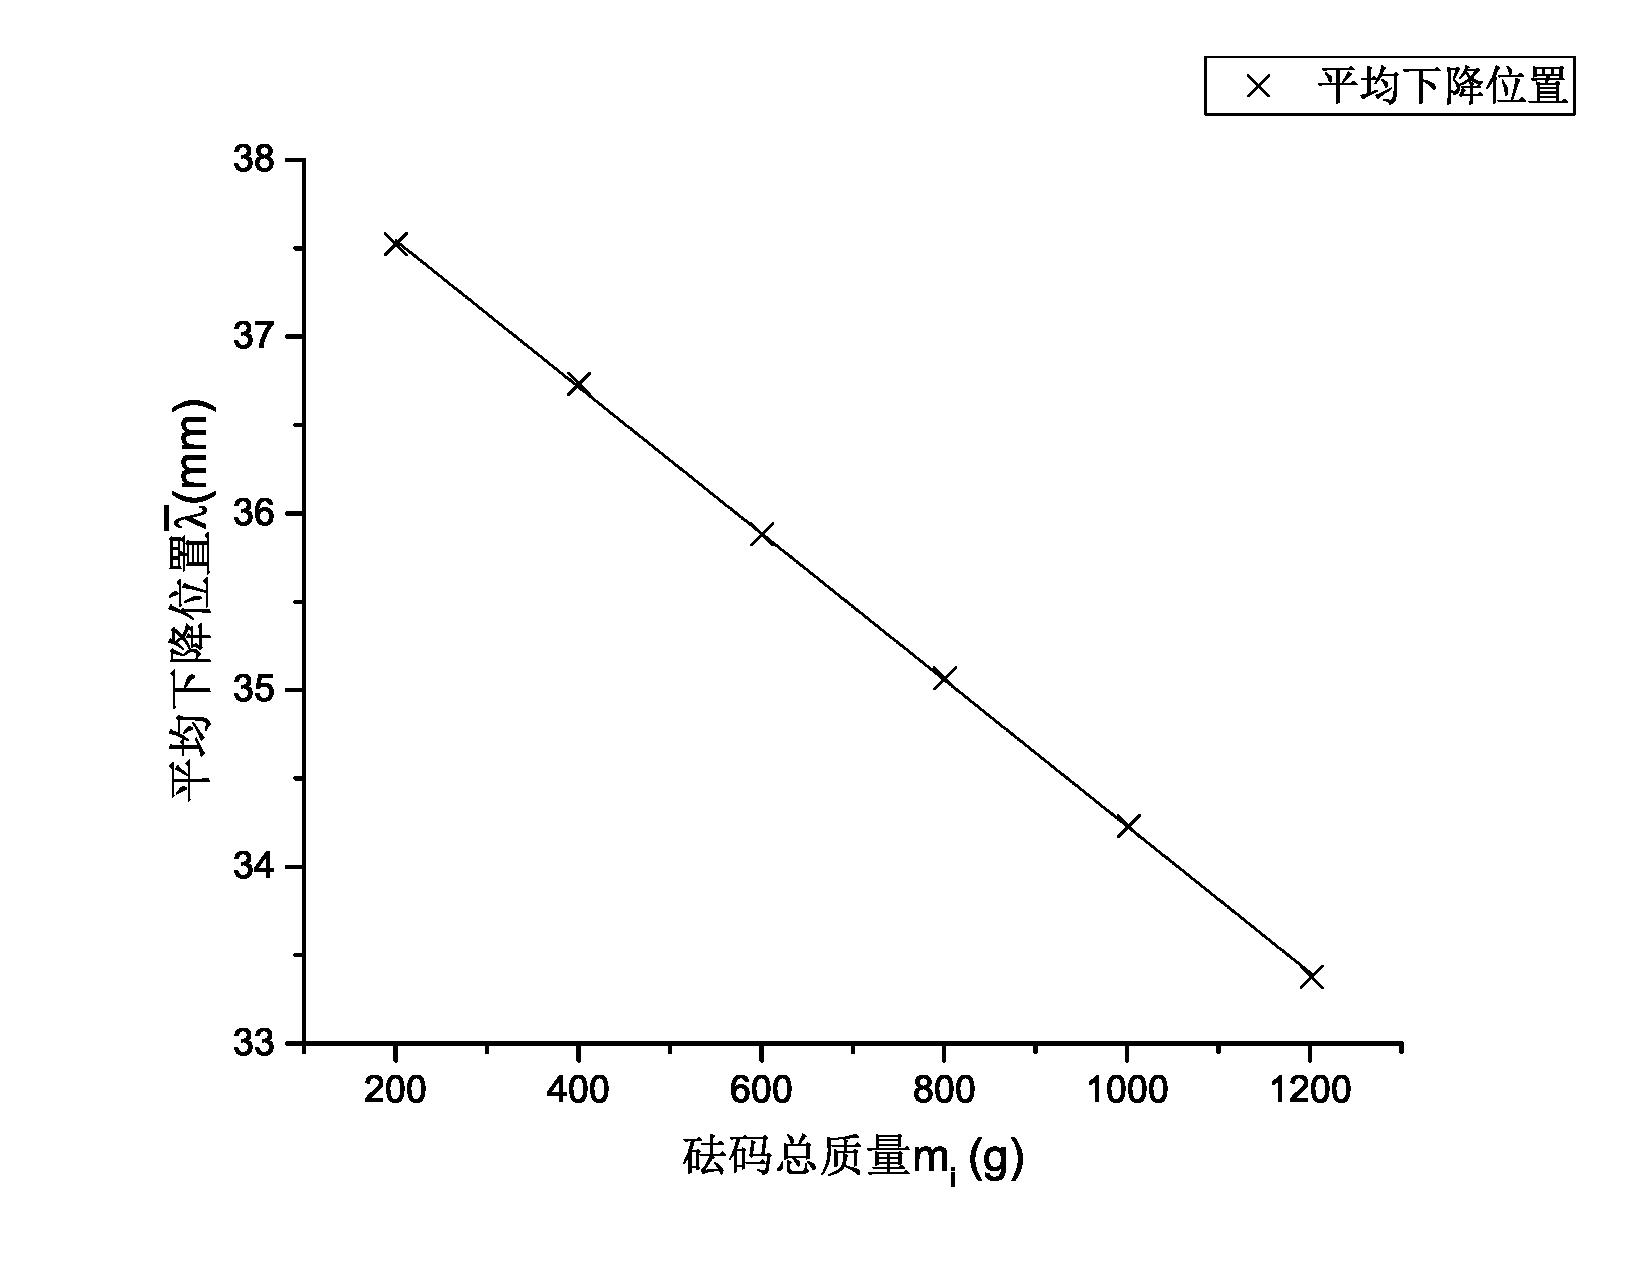
\includegraphics[width=\textwidth]{3}
  \label{fig:digit}
\end{figure}
从图中可以看出,$\bar{\lambda}$与$m$成基本呈线性关系,计算得$\lambda \approx -0.9999$,故确实存在线性关系,下面分别用逐差法和最小二乘法进行数据处理。
\paragraph{逐差法}之前的数据处理中已经计算了各次逐差的值,列表如下:
% Table generated by Excel2LaTeX from sheet 'Sheet3'
\begin{table}[H]
  \centering
  \caption{逐差结果数据表}
    \begin{tabular}{lccc}
    逐差次数  & \multicolumn{1}{l}{$r_0-r_3$} & \multicolumn{1}{l}{$r_1-r_4$} & \multicolumn{1}{l}{$r_2-r_5$} \\
    逐差长度 $\delta \Lambda_i /mm$ & 2.458  & 2.503  & 2.503  \\
    \end{tabular}%
  \label{tab:addlabel}%
\end{table}%

利用公式,有:
$$\delta \Lambda=\frac{1}5 \sum_{i=1}^5{\delta \Lambda_i}=2.488(mm)$$
下计算不确定度:
A类:$$\sigma_{\bar{\Lambda}}=\sqrt{\frac{\sum\limits_{i=1}^3{(\delta \Lambda_i-\overline{\delta \Lambda})^2}}{3\times2}}=0.015(mm)$$
B类:$$e_\Lambda=\sum\limits_{i=1}^3{\frac{e+e}3}=0.008(mm)\Rightarrow \sigma=\frac{e}{\sqrt{3}}=0.005(mm)$$
总不确定度:$$\sigma_\Lambda=\sqrt{\sigma^2+\sigma_{\bar{\Lambda}}^2}=0.016(mm)$$
综上,得;$$\delta \Lambda \pm \sigma_\Lambda=2.488\pm 0.016(mm)$$
\paragraph{最小二乘法}
设$$\bar{\lambda}=k\times m+b$$
考虑到需要计算的物理量,我们对截距进行分析:
$$k=\frac{\sum\limits_{i=0}^5{(\bar{r}_i-\bar{r})(m_i-\bar{m})}}{\sum\limits_{i=0}^5{(m_i-\bar{m})^2}}=-4.14\times 10^{-3}(mm/g)$$
下计算不确定度:
首先计算$\bar{\lambda}$的不确定度:
A类:$$\sigma_r =\sqrt{\frac{1-r^2}{6-2}\sum\limits_{i=0}^9{(\bar{r}_i-\bar{r})^2}}=0.017(mm)$$
B类:$$\sigma=\frac{e+e}{\sqrt{3}}=0.005(mm)$$
总不确定度:$$\sigma_{\bar{r}}=\sqrt{\sigma^2+\sigma_r^2}=0.018(mm)$$
得$k$的不确定度:
$$\sigma_k=\frac{\sigma}{\sqrt{\sum\limits_{i=0}^9{(m_i-\bar{m})^2}}}=2\times10^{-5}(mm/g)$$
故:
$$k\pm \sigma_k=(-4.14\pm 0.02 )\times 10^{-3}(mm/g)$$
\subsection{分别计算金属的杨氏模量}
\subsubsection{利用CCD测量金属的杨氏模量}
原理公式:
$$E=\frac{4mgL}{\pi d^2 \Delta r}$$
\paragraph{逐差法计算}
由于相隔5项逐差,可以将公式改写如下:
$$E=\frac{4\bar{m}gL}{\pi \bar{d}^2 (\frac{\delta L}5)}=1.68\times 10^{11}(Pa)$$
各量不确定度如下:
$$\sigma_m=\sqrt{\frac{\sum\limits_{i=1}^9{(m_i-\bar{m}})^2}{9\times 8}}=0.05(g)$$
$$\sigma_L=0.06(cm)$$
对于金属丝直径:
$$\bar{d}=\frac{1}{10}(\sum_{i=1}^{10}{d_i})-d_0=\bar{d}_{read}-d_0$$
得:
$$\sigma_d=\sqrt{\sigma_{d_{read}}^2+\sigma_{d_0}^2}$$
由于$\sigma_{d_0}$已知,下求$\sigma_{d_{read}}$:
\\
A类:$$\sigma_{\bar{d}}=\sqrt{\frac{\sum\limits_{i=1}^{10}{({d_{read}}_i-\bar{d}_{read})^2}}{10\times9}}=0.0005(mm)$$
B类:$$e_d=\sum\limits_{i=1}^3{\frac{e}3}=0.004(mm)\Rightarrow \sigma=\frac{e}{\sqrt{3}}=0.002(mm)$$
得总不确定度:$$\sigma_{d_{read}}=\sqrt{\sigma_{\bar{d}}^2+\sigma^2}=0.002(mm)$$
得:$$\sigma_d=\sqrt{\sigma_{d_{read}}^2+\sigma_{d_0}^2}=0.003(mm)$$
从而:
$$\sigma_E=\sqrt{(\frac{\partial E}{\partial \bar{m}})^2\sigma_m^2+(\frac{\partial E}{\partial L})^2\sigma_L^2+(\frac{\partial E}{\partial \bar{d}})^2\sigma_d^2(\frac{\partial E}{\partial{(\frac{\delta L}5)} })^2\sigma_{(\frac{\delta L}5)}^2}=0.03\times 10^{11}(Pa)$$
故:$$E\pm \sigma_E=(1.68\pm 0.03)\times 10^{11}(Pa)$$
\paragraph{最小二乘法计算}
由于斜率已知,可将公式改写如下:
$$E=\frac{4gL}{\pi \bar{d}^2 k}=1.69\times 10^{11}(Pa)$$
不确定度计算如下:
$$\sigma_L=0.06(cm)$$
$$\sigma_d=\sqrt{\sigma_{d_{read}}^2+\sigma_{d_0}^2}=0.003(mm)$$
从而:
$$\sigma_E=\sqrt{(\frac{\partial E}{\partial L})^2\sigma_L^2+(\frac{\partial E}{\partial \bar{d}})^2\sigma_d^2+(\frac{\partial E}{\partial k })^2\sigma_k^2}=0.01\times 10^{11}(Pa)$$
故:$$E\pm \sigma_E=(1.69\pm 0.01)\times 10^{11}(Pa)$$
\subsubsection{利用光杠杆测量金属的杨氏模量}
原理公式:
$$E=\frac{8FLR}{\pi d^2 D\Delta r}$$
\paragraph{逐差法计算}
由于相隔5项逐差,可以将公式改写如下:
$$E=\frac{8\bar{m}gLR}{\pi \bar{d}^2 (\frac{\delta L}5 )D}=1.66\times 10^{11}(Pa)$$
\paragraph{最小二乘法计算}
由于斜率已知,可将公式改写如下:
$$E=\frac{8gLR}{\pi \bar{d}^2 kD}=1.65\times 10^{11}(Pa)$$
\subsubsection{梁的弯曲测量金属的杨氏模量}
原理公式:
$$E=\frac{Gl^3}{4 \lambda a h^3}$$
\paragraph{逐差法计算}
由于相隔3项逐差,可以将公式改写如下:
$$E=\frac{\bar{m} g l^3}{4 a h^3 (\frac{\delta \Lambda}3 )}=2.14\times 10^{11}(Pa)$$
\paragraph{最小二乘法计算}
由于斜率已知,可将公式改写如下:
$$E=\frac{gl^3}{4ah^3|k|}=2.14\times 10^{11}(Pa)$$


\section{分析与讨论}
\subsection{$\Delta r$偏大}考虑到开始时钢丝没有拉直,因此,最初的一两个砝码会将金属丝拉直,而在这过程中,相应的$\Delta r$也会偏大。
\subsection{$\Delta r$偏小}若开始时,装置的调节未做好,使得下端圆柱与限转螺丝存在摩擦,则最初时刻的$\Delta r$会因存有摩擦力而较小。
\section{收获和感想}

在课下准备本次实验的时候,我其实并没有感到非常紧张。一来,室友已做过这个实验,可以向他取经;二来,我自己在高中也做过这个实验。

但是,真正实际操作的时候,我却并没有像想象中那般轻松。

一来,进行实验的时候,有一些长度的测量对“身材”提出了要求;二来,我的CCD似乎对我有一些意见……

当然了,结束实验进行总结时,我不由的感叹实验设计的精妙。

在我看来,测量杨氏模量的重要一环,在于将微小的形变放大。无论是搭配了显微镜的CCD,光杆杆还是读数显微镜,都是为了完成这一目标。推而广之,许多实验中,实验设计里都存在着这些将不可观测量转化为可观测量的精妙构想。

在实验课程的学习中,我也要培养自己的实验设计能力,培养自己设计将无法直接测量的物理量进行转化,将低精度测量量转化为高精度的测量量的能力。
    \end{document} 